\documentclass[12pt]{article}
\usepackage[
  paperwidth=16in,
  paperheight=9in,
  margin=0.45in
]{geometry}
\usepackage{amsmath}
\usepackage{xcolor}
\usepackage{enumitem}
\usepackage{tikz}
\usetikzlibrary{arrows.meta,positioning}
\pagestyle{empty}
\setlength{\parindent}{0pt}
\renewcommand{\familydefault}{\sfdefault}

\definecolor{MethodNavy}{HTML}{13294B}
\definecolor{MethodBlue}{HTML}{0072B2}
\definecolor{MethodPurple}{HTML}{7E57C2}
\definecolor{MethodOrange}{HTML}{FF5F05}
\definecolor{MethodTeal}{HTML}{009E73}

\begin{document}
\pagecolor{white}
\color{MethodNavy}

{\fontsize{32}{36}\selectfont\bfseries Methods}

\vspace{0.25in}
\begin{center}
  % Compact poster-ready methods figure.
% Required packages/libraries:
% \usepackage{tikz}
% \usetikzlibrary{arrows.meta,positioning}

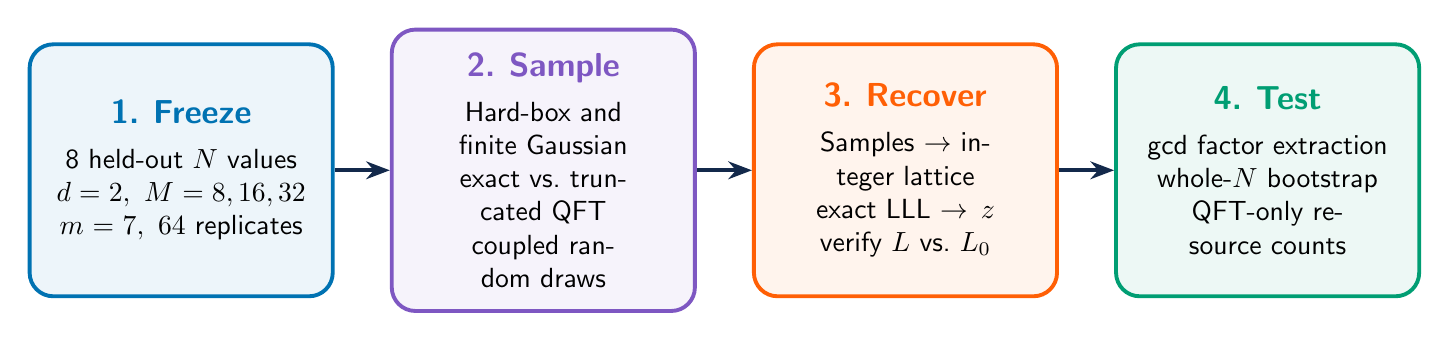
\begin{tikzpicture}[
  font=\sffamily,
  node distance=7mm,
  box/.style={
    rounded corners=3mm,
    draw=#1,
    line width=1.4pt,
    fill=#1!7,
    minimum height=3.2cm,
    text width=3.25cm,
    align=center,
    inner sep=3mm
  },
  arrow/.style={-{Stealth[length=3mm]},line width=1.4pt,draw=MethodNavy}
]
  \node[box=MethodBlue] (freeze) {
    \textcolor{MethodBlue}{\textbf{\large 1. Freeze}}\\[1.5mm]
    8 held-out \(N\) values\\
    \(d=2,\ M=8,16,32\)\\
    \(m=7,\ 64\) replicates
  };

  \node[box=MethodPurple,right=of freeze] (sample) {
    \textcolor{MethodPurple}{\textbf{\large 2. Sample}}\\[1.5mm]
    Hard-box and finite Gaussian\\
    exact vs.\ truncated QFT\\
    coupled random draws
  };

  \node[box=MethodOrange,right=of sample] (recover) {
    \textcolor{MethodOrange}{\textbf{\large 3. Recover}}\\[1.5mm]
    Samples \(\rightarrow\) integer lattice\\
    exact LLL \(\rightarrow z\)\\
    verify \(L\) vs.\ \(L_0\)
  };

  \node[box=MethodTeal,right=of recover] (test) {
    \textcolor{MethodTeal}{\textbf{\large 4. Test}}\\[1.5mm]
    gcd factor extraction\\
    whole-\(N\) bootstrap\\
    QFT-only resource counts
  };

  \draw[arrow] (freeze) -- (sample);
  \draw[arrow] (sample) -- (recover);
  \draw[arrow] (recover) -- (test);
\end{tikzpicture}


\end{center}

\vspace{0.18in}
\begin{minipage}[t]{0.64\linewidth}
  % Paste this file inside the Methods block of your poster.
% Required packages in the poster preamble:
% \usepackage{amsmath}
% \usepackage{xcolor}
% \usepackage{enumitem}

\definecolor{MethodNavy}{HTML}{13294B}
\definecolor{MethodBlue}{HTML}{0072B2}
\definecolor{MethodPurple}{HTML}{7E57C2}
\definecolor{MethodOrange}{HTML}{FF5F05}
\definecolor{MethodTeal}{HTML}{009E73}

\begin{minipage}{\linewidth}
\color{MethodNavy}
\textbf{\large Research question.}
Does removing the smallest controlled-phase rotations from the inverse
quantum Fourier transform (QFT) preserve factor recovery at the complete
finite Regev-style lattice endpoint?

\vspace{0.45em}
\begin{enumerate}[leftmargin=1.45em,itemsep=0.45em,topsep=0.2em]
  \item[\textcolor{MethodBlue}{\textbf{1}}]
  \textbf{Freeze the test.}
  We fixed eight held-out semiprimes,
  \(d=2\), stored roots \((b_1,b_2)=(2,3)\),
  Fourier moduli \(M\in\{8,16,32\}\), \(m=7\) samples,
  64 coupled replicates per cell, and master seed \(2026071301\).

  \item[\textcolor{MethodPurple}{\textbf{2}}]
  \textbf{Generate exact finite Fourier samples.}
  We evaluated both the notebook's uniform hard-box state and an exact finite
  discrete-Gaussian state with \(R=4\).
  Each condition used either the exact inverse QFT or a distance-truncated
  inverse QFT that removes the smallest-angle phase layers.

  \item[\textcolor{MethodOrange}{\textbf{3}}]
  \textbf{Run the complete classical endpoint.}
  Measured samples were converted to an augmented integer lattice, reduced
  with exact LLL, and lifted to candidate relations \(z\).
  We verified
  \[
    \prod_i a_i^{z_i}\equiv 1\pmod N,
    \qquad a_i=b_i^2\bmod N,
  \]
  then used the stored roots \(b_i\) to distinguish useful
  \(L\setminus L_0\) relations and extract factors with a gcd.

  \item[\textcolor{MethodTeal}{\textbf{4}}]
  \textbf{Compare exact and truncated QFTs.}
  Exact and truncated conditions used coupled random draws.
  Factor-recovery differences were aggregated with \(N\), not repeated
  trials, as the unit of generalization.
  A 5,000-draw whole-\(N\) cluster bootstrap tested the frozen
  \(-0.10\) non-inferiority margin.
  We separately counted QFT-only controlled-phase gates, transpiled CX gates,
  and depth.
\end{enumerate}

\vspace{0.35em}
\colorbox{MethodNavy}{%
  \parbox{\dimexpr\linewidth-2\fboxsep\relax}{%
    \centering\color{white}\small
    Known factors were never used for sampling, tuning, or relation
    classification; they were used only for post-hoc validation.
  }%
}
\end{minipage}


\end{minipage}\hfill
\begin{minipage}[t]{0.32\linewidth}
  \colorbox{MethodPurple!8}{%
    \parbox{\dimexpr\linewidth-2\fboxsep\relax}{%
      \textbf{\large Frozen parameters}\\[1mm]
      \(\displaystyle N\in
      \{55,65,85,95,115,119,133,161\}\)\\[1mm]
      Stored roots: \((2,3)\)\\
      \(d=2,\ M\in\{8,16,32\},\ m=7\)\\
      Gaussian radius: \(R=4\)\\
      64 coupled replicates per cell\\
      5,000 whole-\(N\) bootstrap draws\\
      Primary margin: \(0.10\)
    }%
  }

  \vspace{0.18in}
  \colorbox{MethodOrange!8}{%
    \parbox{\dimexpr\linewidth-2\fboxsep\relax}{%
      \textbf{\large What this is not}\\[1mm]
      This is a finite exact simulation study of QFT phase truncation.
      It is not calibrated hardware noise, cryptographic-scale factoring,
      or an end-to-end speedup benchmark.
    }%
  }
\end{minipage}

\end{document}
